\section{Birth and death Markov processes}
We discuss here a simple class of Markov processes, those that have a set of states that can be labeled with integers. We start from an even simpler discrete Morkor process, the binth and deoth processes which occur in mony applications. Then we will deduce results to more general coses.
We otact from a rituation that is very similar to the zondom wolk. We assume discrete times $t=0, \Delta t, 2 \Delta t, \ldots$ discrete states $x=0, \pm 1, \pm 2 \ldots$ and that jumps are allowed only between nearest neighbors, i.e. from $n$ to $n \pm 1$. For $\Delta t \ll 1$ we call $b_{n} \geqslant 0$ the birth wate, i.e., $b_{n} \Delta t$ is the prob. to jump to $n+1$ at time $t+\Delta t$, given that at time $t$ the state was $n$. (notice that $b_{n}$ daes not depend on time, thangh it cauld in principle. If it does not, we say that the process is homogeneous). Analogously, $d_{n} \geqslant 0$ is the death rate, i.e. $d_{n} \Delta t$ is the prob. to jump to $n-1$ at time $t+\Delta t$, given that at time $t$ the strate was $n$.
We want to calculate the prob. $p(n, t+\Delta t)$ (the propagotor).
\begin{center}
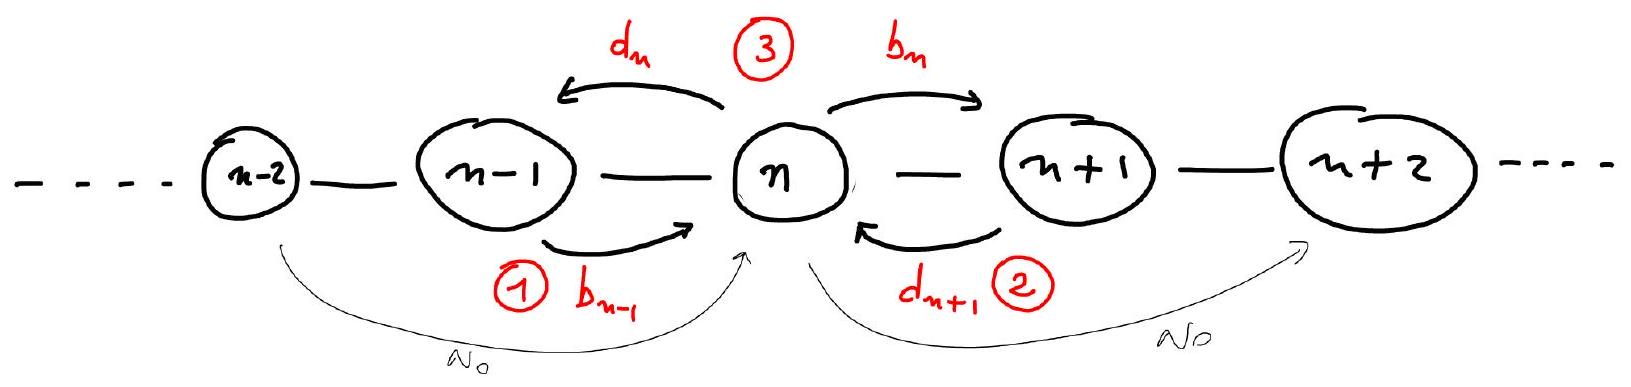
\includegraphics[width=\textwidth]{2025_10_17_3daf2a002a8f5936c90eg-01}
\end{center}


\begin{equation*}
p(n, t+\Delta t)=b_{n-1} \Delta t p(n-1, t)+d_{n+1} \Delta t p(n+1, t)+\left[1-\left(b_{n}+d_{n}\right) \Delta t\right] p(n, t) \tag{1}
\end{equation*}


By Taylor exponsions and then taking the limit $\Delta t \rightarrow 0$ we get
(1) $\quad \frac{\partial p_{n}}{\partial t}=b_{n-1} p_{n-1}(t)+d_{n+1} p_{m+1}(t)-\left(b_{n}+d_{n}\right) p_{n}(t)$

This is called the moster equation of the binth-deoth process or generation-riconlaination process.

A few observations:

\begin{enumerate}
  \item The M.E. is a gain-loss equation for the probabilities $p_{n}$;
  \item We have to equip ey. (1) with imitial conditions. If We start with $P_{n, n_{0}}\left(t_{0}\right)=\delta_{m_{1} m_{0}}$, then the M.E. is the equation of the propogator of the Mackov process, that is
\end{enumerate}

$$
 P_{n}(t) \equiv P\left(n, t \mid n_{0} t_{0}\right)
$$ 

So ane con show (exercize) that $p_{n}(t)$ satisfies the ChapmanKolmogozov ep. in its obfferential form. More fallows on this.
\begin{enumerate}
\setcounter{enumi}{2}
  \item We con introduce boundary conditions as well. For instance, if $N$ is a reflecting boundary,
\end{enumerate}
(2)
\begin{center}
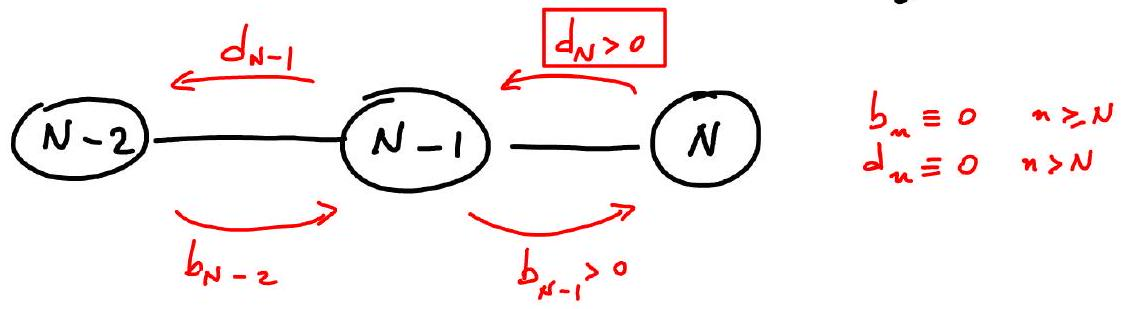
\includegraphics[width=\textwidth]{2025_10_17_3daf2a002a8f5936c90eg-02}
\end{center}
then $b_{n} \equiv 0 \forall n \geqslant N, d_{n} \equiv 0 \forall n>N \quad\left(\right.$ for $n<N, b_{n}$ and $d_{n}$ ore $\left.\geqslant 0\right)$ therefore if the state $N$ is reached, it can be left from one side only. $N$ is a reflecting state.

If $N$ is ar absolsing boundry,
(3)
\begin{center}
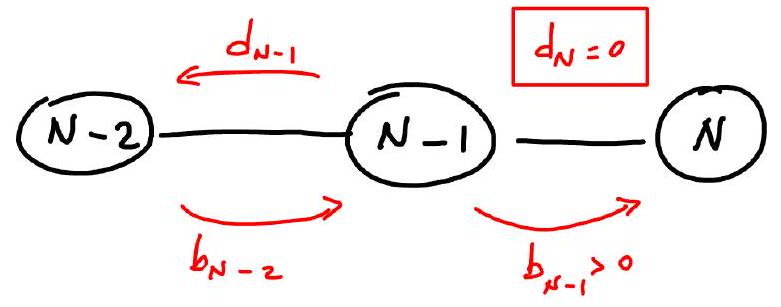
\includegraphics[width=\textwidth]{2025_10_17_3daf2a002a8f5936c90eg-03}
\end{center}
here $d_{N}=0$ which is important, because when the state $N$ is reached, it con no longer be left. We say that $N$ is an absorbing state.

\section*{Warning:}
Because of the b.c. We have to be coreful with ep. (1) as it holds only when the boundory states are not hit, otherwise it must be changed.
\begin{enumerate}
\setcounter{enumi}{3}
  \item Notice that ep. (1) is limeor and deterministic; indeed we con define a matrix $\mathbb{W}$ whose entries are
\end{enumerate}
(4a) $\mathbb{W}_{m m^{\prime}}=d_{m^{\prime}} \delta_{m, m^{\prime}-1}+b_{m^{\prime}} \delta_{m, m^{\prime}+1}-\left(d_{m}+b_{m}\right) \delta_{m, n^{\prime}}$

So, if we introduce the vector notation $[\vec{p}(t)]_{n} \equiv p_{n}(t)$ we con write ef. (1) as
(4b) $\quad\left\{\begin{array}{l}\dot{\vec{P}}(t)=\mathbb{W} \vec{P} \\ \vec{P}(0)=\vec{P}_{0}\end{array}\right.$
and formally the solution reads $\vec{P}(t)=e^{\mathbb{W} t} \vec{P}_{0}$.
The moster equation defined in ep. (4b) holds in general for a continuous time, discrete Morkov process as long as $\mathbb{W}$ sotisfies the following properties:

\begin{enumerate}
  \item $W_{n x^{\prime}} \geqslant 0$ for $n \neq n^{\prime}$
  \item $\sum_{m} \mathbb{W}_{m n^{\prime}}=0$ for each $n^{\prime}$ (no abs. bound.)
\end{enumerate}

The equations for the mean and the variance Frome op. (1) One con simply desive the eps. for the fine evolution of the mean and the verionce. We first multiply of. (1) by $x$ and sum over $x$: $\langle n\rangle \equiv \sum_{-\infty}^{+\infty} n p_{n}(t)$

$$ 
\begin{aligned}
\frac{d}{d t}\langle n\rangle & =\sum_{-\infty}^{+\infty}\left(n b_{n-1} p_{n-1}-n b_{n} p_{n}+n d_{n+1} p_{n+1}-n d_{n} p_{n}\right) \\
& =\sum_{n}\left[(n+1) b_{n} p_{n}-n b_{n} p_{n}+(n-1) d_{n} p_{n}-n d_{n} p_{n}\right] \\
& =\sum_{n}\left(b_{n}-d_{n}\right) p_{n}
\end{aligned}
$$ 

(5)

$$ 
\begin{array}{ll}
\frac{d}{d t}\langle n\rangle=\left\langle b_{n}\right\rangle-\left\langle d_{n}\right\rangle & \left\langle b_{n}\right\rangle \equiv \sum_{n} b_{n} p_{n} \\
 & \left\langle d_{n}\right\rangle \equiv \sum_{n} d_{n} p_{n}
\end{array}
$$ 

with some initial conditions. Notice that this equation has to be opuipped with different equations if there is an absorbing or reflecting b.c. Can you find them?

For the evolution of the verionce we have to desive an equation for the second moment $\left\langle n^{2}\right\rangle$. We first multiply ep. (1) by $n^{2}$ and then sum over $n$ :

$$ 
\begin{aligned}
\frac{d}{d t}\left\langle n^{2}\right\rangle & =\sum_{-\infty}^{+\infty} n^{2}\left(b_{m-1} p_{m-1}+\cdots\right)=\\
& =\sum_{m}\left((n+1)^{2}-n^{2}\right) b_{m} p_{m}+\sum_{m}\left[(n-1)^{2}-n^{2}\right] d_{m} p_{m} \\ & =\sum_{m}(2 n+1) b_{m} p_{m}+\sum_{m}(-2 n+1) d_{m} p_{m} \\ & =2 \sum_{m} n\left(b_{m}-d_{m}\right) p_{m}+\sum_{m}\left(b_{m}+d_{m}\right) p_{m}
\end{aligned}
$$ 

Thus
(6) $\frac{d}{d t}\left\langle m^{2}\right\rangle=2\left\langle n\left(b_{n}-d_{n}\right)\right\rangle+\left\langle b_{n}+d_{n}\right\rangle$

The equilibrium distribution
For binth and deoth procen it is possible to colculate the equilibrium distribution of ef. (1) in general. This is not possible for more complicated discrete Marker processes.
We will colulate the distribution for a $b/d$ process defined between O (2.b.c.) and $\infty$.
We con define a stationary flux from $n-1$ to $n$ :
\begin{center}
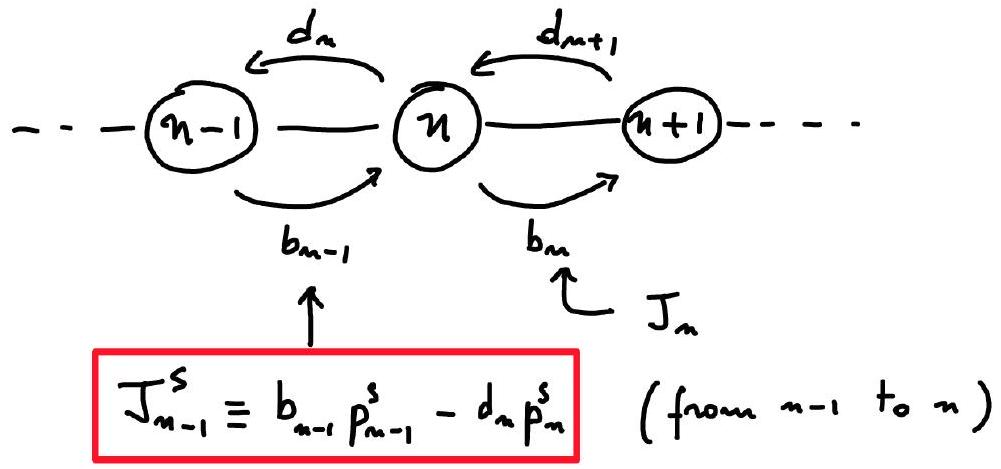
\includegraphics[width=0.5\textwidth]{2025_10_17_3daf2a002a8f5936c90eg-05}
\end{center}

From ep. (1) we get then

$$ 
 0=\underbrace{b_{n-1} p_{n-1}^{s}-d_{n} p_{n}^{s}}_{J_{n-1}}+\underbrace{d_{n+1} p_{n+1}^{s}-b_{n} p_{n}^{s}}_{-J_{n}}
$$ 

hence $J_{m}=J_{m-1}=\ldots=J_{0} = b_{-1} p_{-1}^{s}-d_{0} p_{0}^{s}=0$ Truff.b.c. at $m=0$
then

$$ 
\begin{gathered}
J_{n}=b_{n-1} p_{n-1}^{s}-d_{n} p_{n}^{s}=0 \Rightarrow b_{n-1} p_{n-1}^{s}=d_{n} p_{n}^{s} \quad \text{DETAILED BALANCE} \\
p_{n}^{s}=\frac{b_{n-1}}{d_{n}} p_{n-1}^{s}=\frac{b_{n-1}}{d_{n}} \frac{b_{n-2}}{d_{n-1}} p_{n-2}^{s}=\ldots
\end{gathered}
$$ 

(7) $\quad p_{m}^{s}=\prod_{1}^{n} \frac{b_{i-1}}{d_{i}} p_{0}^{s} \quad$ for $n=1,2, \ldots$
becouse of normolizetion, $\left(p_{0}^{s}\right)^{-1}=1+\sum_{1}^{\infty} \prod_{i}^{\infty} \frac{b_{i-1}}{d_{i}}$; $p_{i}^{s}$ exists if $p_{0}^{s}<\infty$. The some approach can be used for a finite number of states $n=1, \ldots, N$.

\section*{Simple yet important birth and death processes}
Poisson process
This procen is defined by the sotes $b_{n}=\lambda, d_{n}=0$, where $n=0,1, \ldots$ So the $M-E$. is
(8) $\quad\left\{\begin{array}{l}\dot{p}_{m}=\lambda\left(p_{m-1}-p_{m}\right) \\ p_{m}(0)=\delta_{m, 0}\end{array}\right.$

Ex: show that the mean sotisfies the eq. $\frac{d}{d t}\langle u\rangle=\lambda$ and so $\langle n(t)\rangle=n_{0}+\lambda t$ if $p_{n}(0)=\delta_{n, n_{0}}$.

We solve op. (8) with the method of the generating function:

$$ 
 g(z, t) \equiv \sum_{0}^{\infty} z^{n} p_{n}(t)
$$ 

So from ep. (8) we get an ef. for $g$ :
(9) $\quad\left\{\begin{array}{l}\frac{\partial}{\partial t} g(z, t)=\lambda(z-1) g(z, t) \quad\left(g(1, t)=\sum_{n} p_{n}(t)=1\right) \\ g(z, 0)=\sum_{n} z^{n} \delta_{n, 0}=1\end{array}\right.$

The solution of (3) is then


\begin{equation*}
 g(z, t)=e^{\lambda(z-1) t}=e^{-\lambda t} \overbrace{\sum_{0}^{\infty} \frac{(\lambda t)^{n}}{n!} z^{n}}^{e^{\lambda z}}=\sum_{0=n}^{\infty} p_{n}(t) z^{n} \tag{8}
\end{equation*}


hence
(10) $p_{n}(t)=e^{-\lambda t} \frac{(\lambda t)^{n}}{n!}$

Show that $\operatorname{var}(n(t))=\lambda t$.

Radioactive decay
Unitially the rystem consists of $N_{0}$ sodioactive porticles which decay at sate $\gamma$. Therefore, if at time $t$ there are $n$ surviving perticles, then in the following $\Delta t$ time the probability of one decay is $\gamma n \Delta t$ and more thon one decay is $\sigma(\Delta t)$. Thus $d_{n}=\gamma n$ and $b_{n}=0$ and the M.E. is

$$ 
\left\{\begin{array}{l}\dot{p}_{n}=\gamma(n+1) p_{n+1}(t)-\gamma m p_{n}(t) \quad n=0,1 \ldots N_{0}-1 \quad \text{a.b.c. at } n=0 . \\ \dot{p}_{N_{0}}=-\gamma N_{0} p_{N_{0}}(t) \\ p_{n}(0)=\delta_{n, N_{0}}\end{array}\right.
$$ 

Ex: show that $\frac{d}{d t}\langle n\rangle=-\gamma\langle n\rangle$, so $\langle n(t)\rangle=N_{0} e^{-\gamma t}$.
With the generating function $g(z, t)=\sum_{0}^{N_{0}} z^{n} p_{n}(t)$ we get

$$ 
 \text { (11) } \quad \frac{\partial g(z, t)}{\partial t}=\gamma(1-z) \frac{\partial}{\partial z} g(z, t) \quad \begin{aligned} & g(1, t)=1 \\ & g(z, 0)=z^{N_{0}} \end{aligned}
$$ 

Notice that $h\left(z_{1} t\right)=\varepsilon(t)(1-z)+1$ leads to $\varepsilon=-\gamma \varepsilon$, namely $\varepsilon(t)=\varepsilon_{0} e^{-\gamma t}$, so $h(1, t)=1$, but $h(z, 0)=\varepsilon_{0}(1-z)+1 \neq z^{N_{0}}$. However, take $g$ as a function of $h$, i.e. $g(z, t)=f(h(z, t))$, we get from (11)

$$ 
\frac{\partial g}{\partial t}=\frac{d f}{d h} \frac{\partial h}{\partial t} \quad , \quad \frac{\partial g}{\partial z}=\frac{d f}{d h} \frac{\partial h}{\partial z}
$$ 

and $\frac{d f}{d h}$ simplifies, because it occurs on both sides of ey. (11). We con then use $f$ to satisfy the i.c.: $f(a)=a^{N_{0}}$ does the job. We take $g=\left(\varepsilon_{0} e^{-\gamma t}(1-z)+1\right)^{N_{0}}$ where $\varepsilon_{0}=-1$. Eventually, the sol, is
(12) $g(z, t)=\left(e^{-\gamma t}(z-1)+1\right)^{N_{0}}$

We have now to invect this relation to get $p_{n}(t)$
$g(z, t)=\left(e^{-\gamma t} z+\left(1-e^{-\gamma t}\right)\right)^{N_{0}}=\sum_{0}^{N_{0}}\binom{N_{0}}{m}\left(1-e^{-\gamma t}\right)^{N_{0}-n} e^{-n \gamma t} z^{n}$
which gives
(13) $\quad p_{n}(t)=\binom{N_{0}}{n} e^{-n \gamma t}\left(1-e^{-\gamma t}\right)^{N_{0}-n}$

We con interpret this ep. in this way: $e^{-n \gamma t}$ is the prob. that $n$ particles have survived (i.e., not decayed yet) by time $t,\left(1-e^{-\gamma t}\right)^{N_{0}-n}$ is the prob. that $N_{0}-n$ porticles have decayed by time $t$. We also need the factor $\binom{N_{0}}{n}$ because the specific identity of the porticles is not important, then there ore $\binom{N_{0}}{n}$ Ways to select $n$ surviving particles out of $N_{0}$.

\section*{Furry process}
A cosmic electron enters an absorbing material (like lead...) and branches into multiple particles (an electron may emit a photon which moy then preduce an $e^{+}-e^{-}$poir). So a coscode of secondory poiticles is produced which generotes a shower of final porticles. This process can be deserved by a birth and death procen where $b_{n}=\gamma n$ and $d_{n}=0, n=1,2, \ldots$
The M.E. is then

$$ 
\left\{\begin{array}{l}\dot{p}_{n}=\gamma(n-1) p_{n-1}-\gamma n p_{n} \\ p_{n}(0)=\delta_{n, 1}\end{array}\right.
$$ 

Show as before that

$$ 
\begin{aligned}
& \langle n(t)\rangle=e^{\gamma t} \\
& \operatorname{Var}(n(t))=e^{\gamma t}\left(e^{\gamma t}-1\right)
\end{aligned}
$$ 

Finally:
(14) $\quad p_{n}(t)=e^{-\gamma t}\left(1-e^{-\gamma t}\right)^{n-1}$ try to interpet the vesult.

\section*{The contect procen}
Let us assume that a population of $N$ individuals can be devided into two cotegories according to whether they are infected on not (but are susceptible any way). If an indiv. has not yet cought the infection, may catch it from any of of the $n$ infected ones (uniformly at random).
We con write down the trousition rote from $n$ to $n+1$ infected individuals; if the number of infected ind. increases by one, then one healthy ind. must get in conctact with an infected one:

\begin{enumerate}
  \item finst, we have to pick one healthy indiv.
\end{enumerate}

$$ b_{n}=\tilde{\beta} \frac{N-n}{N} \frac{n}{N-1}=\frac{\beta}{N} n(N-n) $$ 

\begin{enumerate}
  \setcounter{enumi}{1}
  \item second, the healthy ind. have to encounter an infected one.
\end{enumerate}

We then assume that an infected individual recovers at rote $\gamma$. then the trousition rote from state $n$ to $n-1$ is $d_{n}=\gamma n$. Notice that $b_{0}=0=d_{0}$ ( $n=0$ is an assorbing state) and $b_{N}=0, d_{N} \neq 0 \quad (n=N$ is a reflecting state $)$ and we have to set $d_{N+1}=0$.
Notice that the zotes $b_{n}$ and $d_{n}$ con be written as a function of $x=\frac{n}{N}: b_{x}=N \beta x(1-x), d_{x}=N \gamma x$.
As $N$ becomes large, the variations in $n$ become surall and so one hopes to describe $x$ as a continuous variable. Making this limit rigorous is tricky (Kurtz's theorem), but one con anywoy guess the limiting guation. the important assumption is the existence of a typical scale of the system (in this cose $N$ ) and that the perameters (here $\beta$ and $\gamma$ ) scale appropriately with $N$.

The master equation has a form
(15) $\quad \dot{q}_{n}(t)=b_{\frac{n-1}{N}} q_{n-1}+d_{\frac{n+1}{N}} q_{n+1}-\left(b_{\frac{n}{N}}+d_{\frac{n}{N}}\right) q_{n}$

In the continuous limit $q_{u}(t)$ becomes a $P D F$ of $x, s_{0}$ we write

$$ q_{n}(t)=\frac{1}{N} p(x, t) \quad \text { for lorge } N $$ 

So eq. (15) becomes
(16)
$\dot{p}(x, t)=b_{x-\frac{1}{N}} p\left(x-\frac{1}{N}, t\right)+d_{x+\frac{1}{N}} p\left(x+\frac{1}{N}, t\right)-\left(b_{x}+d_{x}\right) p(x, t)$

As $\frac{1}{N}$ is surall, we con Taylar expand $\varphi$. (16):

$$ 
\begin{aligned}
& b_{x-\frac{1}{N}} p\left(x-\frac{1}{N}\right)-b_{x} p(x)=-\frac{1}{N} \frac{d}{d x}\left(b_{x} p_{x}\right)+\frac{1}{2} \frac{1}{N^{2}} \frac{d^{2}}{d x^{2}}\left(b_{x} p_{x}\right)+\text { h.o.t. } \\
& d_{x+\frac{1}{N}} p\left(x+\frac{1}{N}\right)-d_{x} p(x)=\frac{1}{N} \frac{d}{d x}\left(d_{x} p_{x}\right)+\frac{1}{2} \frac{1}{N^{2}} \frac{d^{2}}{d x^{2}}\left(d_{x} p_{x}\right)+\text { h.o.t. }
\end{aligned}
$$ 

Therefore
(17) $\dot{p}(x, t)=-\frac{1}{N} \frac{\partial}{\partial x}\left[\left(b_{x}-d_{x}\right) p_{x}\right]+\frac{1}{2 N^{2}} \frac{\partial^{2}}{\partial x^{2}}\left[\left(b_{x}+d_{x}\right) p_{x}\right]+$ h.o.t. as $b_{x}=N \beta x(1-x)$ and $d_{x}=N \gamma x$ we get the F.P. equation
(18) $\dot{p}(x, t)=-\frac{\partial}{\partial x}[(\beta x(1-x)-\gamma x) p]+\frac{1}{2 N} \frac{\partial^{2}}{\partial x^{2}}[(\beta x(1-x)+\gamma x) p]$
which corresponds to an Ita SDE: ( $0<x<1$ )
(18b) $d x=(\beta x(1-x)-\gamma x) d t+\sqrt{\frac{\beta x(1-x)+\gamma x}{N}} d B(t)$
Fluctuotions are of order $N^{-1 / 2}$.

On general, although the equation and its derivation are not rigorous, a binth and deoth process may be well approximated by the F.P. equation
(19)

$$ 
\dot{p}(x, t)=-\frac{\partial}{\partial x}\left[\left(b_{x}-d_{x}\right) p_{x}\right]+\frac{1}{2} \frac{\partial^{2}}{\partial x^{2}}\left[\left(b_{x}+d_{x}\right) p_{x}\right]
$$ 
at least in some region of the porometer space. It is anywey expected that ef. (19) is very imaccurate close to (possible) boundaries or when $N$ (or other typical powar.) is small. This approx is called Kramers-Moyal expension and has several generalizations. Other more rigorous approximations exist (like the von Kompen approximation (see p. 244, ven Kompen) or the WKB expension... which are more accurate but more difficult as well.

Back to the contact process.
The mean of the infected individuals, $\rho(t) \equiv \mathbb{E}(x(t))$, sotisfies (see e. (18b)

(20) $\dot{\rho}=(\beta-\gamma) \rho-\beta \mathbb{E}\left(x(t)^{2}\right)$

This equation is not clased and cammot be solved, unlen we know the behavior of $\mathbb{E}\left(x^{2}\right)$. The mean depends on the fluctuations. However, the ep. for $\mathbb{E}\left(x^{2}\right)$ depends on $\mathbb{E}\left(x^{3}\right)$, so we obtain an infinite choin of equations which comot be solved unless we solve the full F.P. equation.
One way to obtain some information is to resort to the moment clasure: if fluctuations are small, then

$$ 
\mathbb{E}\left(x^{2}(t)\right) \simeq \mathbb{E}(x(t))^{2}=\rho(t)^{2}
$$ 

Under this approximation
(21) $\quad \dot{\rho}=(\beta-\gamma) \rho-\beta \rho^{2}$
which is a logistic equation that can be solved as we have seen at the beginning of the course.
There are two steady states $(\dot{\rho}=0): \rho^{*}=0$ and $\bar{\rho}=\frac{\beta-\gamma}{\beta}$. What is their meoming?
Let's look at their stability:

$$ 
\frac{d \dot{\rho}}{d \rho}=\beta-\gamma-\left.2 \beta \rho\right|_{\rho=\rho^{s t}}=\left\{\begin{array}{cc}
\beta-\gamma & \rho=\rho^{*}=0 \\ \gamma-\beta & \rho=\bar{\rho}=\frac{\beta-\gamma}{\beta}\end{array}\right.
$$ 

\begin{itemize}
  \item Therefore $\rho=0$ is stable as $\beta<\gamma$ (and $\bar{\rho}$ is unstable)
\begin{center}
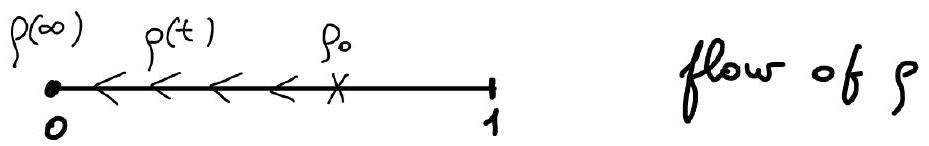
\includegraphics[width=0.5\textwidth]{2025_10_17_3daf2a002a8f5936c90eg-12}
\end{center}
after some time, the ey. is well approximoted by
\end{itemize}

$$ 
\dot{\rho}=(\beta-\gamma) \rho \quad \rightarrow \rho(t)=\tilde{\rho} e^{-|\beta-\gamma| t} \rho \rightarrow_{t}
$$ 

\begin{itemize}
  \item Viceversa, $\bar{\rho}=\frac{\beta-\gamma}{\beta}(>0)$ is stable as $\beta>\gamma$ (and $\rho=0$ is unstable)
\begin{center}
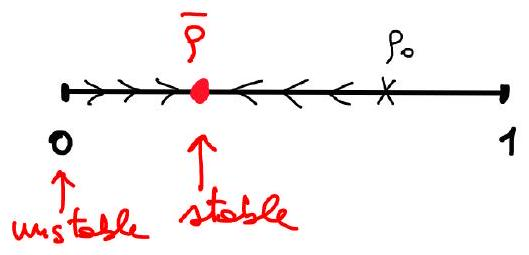
\includegraphics[width=0.5\textwidth]{2025_10_17_3daf2a002a8f5936c90eg-12(1)}
\end{center}
ofter some time, the ef. is well approximated by $\rho(t)=\bar{\rho}+y(t)$ ( $y \ll \bar{\rho}$ )
\end{itemize}

$$ 
\dot{\rho}=-(\beta-\gamma)(\bar{\rho}-\rho) \quad \rightarrow \quad \rho(t)=\bar{\rho}+\tilde{\rho} e^{-|\beta-\gamma| t}
$$ 

$$ 
\begin{center}
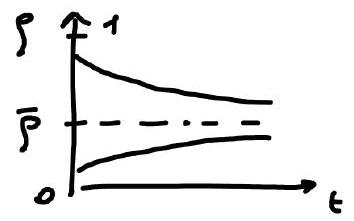
\includegraphics[width=0.5\textwidth]{2025_10_17_3daf2a002a8f5936c90eg-12(2)}
\end{center}
$$ 

So the characteristic time scale is $|\beta-\gamma|^{-1}$ in both coses.
of consse this is summorized by the full solution:
(22) $\quad \rho(t)=\frac{\bar{\rho}}{1+\left(\frac{\bar{\rho}}{\rho_{0}}-1\right) e^{(\gamma-\beta) t}}=\frac{(\beta-\gamma) \rho_{0}}{\beta \rho_{0}+\left(\beta-\gamma-\beta \rho_{0}\right) e^{(\gamma-\beta) t}}$
where $\rho_{0}$ is the initial condition for the deusity $\left(0<\rho_{0}<1\right)$ of infected individuals.
The phose digram of this process reads :
\begin{center}
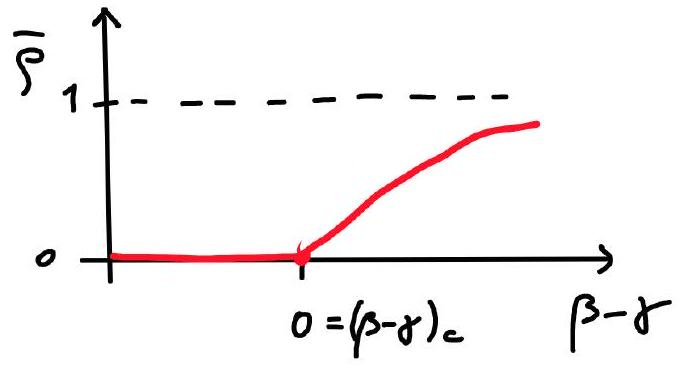
\includegraphics[width=0.5\textwidth]{2025_10_17_3daf2a002a8f5936c90eg-13}
\end{center}

$$ 
\begin{gathered}
\bar{\rho} \sim(\beta-\gamma)^{1} \\
\beta>\gamma
\end{gathered}
$$ 

At the critical point $\beta=\gamma$ :

$$ 
\dot{\rho}=-\beta \rho^{2} \quad \rightarrow \quad \rho(t)=\frac{\rho_{\infty}}{1+\beta t} \sim \frac{1}{t} \quad t \gg \beta^{-1}
$$ 
the decay is no longer exponential but power law : critical slowing down.

Exercife: the discrete zondom walk in continuous time is governed by the master equation (symmetric R.W.)

$$ 
\dot{p}_{n}=p_{n+1}+p_{n-1}-2 p_{n} \quad p_{n}(0)=\delta_{n, 0}
$$ 

Show that the generating function $F(z, t)=\sum_{-\infty}^{+\infty} z^{n} p_{n}(t)$ satisfies

$$ 
\dot{F}=\left(z+\frac{1}{z}-2\right) F
$$ 

so the solution is $F(z, t)=\exp \left[t\left(z+z^{-1}-2\right)\right]$. From this find

$$ p_{n}(t)=e^{-t} \sum_{\substack{l \geqslant 0 \\ l+m \geqslant 0}} \frac{t^{2 l+m}}{(l+m)!l!}
$$ 

Find the K.M. exponsion of the T.E. and find its solution.

A simple chemical reaction
Consider the reaction

$$ X \underset{k_{2}}{\stackrel{k_{1}}{\rightleftarrows}} A
$$ 
where the product $A$ is not affected by $x$ and it does not decrease its quontity even though it produces porticles at wate $k_{2}$. We ore interested into the stochastic evolution of $X$ : the $2 . v . n$. From a simple application of the mass action law we get the evolution of the deterministic value $\rho(t)=\mathbb{E}(n(t))$ :
(23) $\quad \dot{\rho}=-k_{1} \rho+k_{2} a \quad a$ is a constant.

We wont now to get imponestion obout the fluctuations: If at time $t$ there are $n$ particles of type $x$, then the prob. that at time $t+\Delta t$ there is one more is given by $k_{2} a \Delta t$, and one less is $k_{1} n \Delta t$. So we get a binth and death process with zotes

$$ 
\begin{aligned}
& b_{n}=k_{2} a \equiv b \quad(\text { a constant }) \\
& d_{n}=k_{1} n
\end{aligned}
$$ 
where $n=0,1, \ldots$
at is not difficult to find that the equilibrium distribution of $x$ (from ep. (7))
(24) $\quad p_{n}^{s t}=\frac{\lambda^{n}}{n!} e^{-\lambda} \quad \lambda=\frac{k_{2}a}{k_{1}}$
what is the difference between this solution and ep. (10)?
The average is also (from ep. (5))

$$ 
\frac{d}{d t}\langle x\rangle=b-k_{1}\langle x\rangle
$$ 
which is like e. 23 .
Ex: find the M.E. for the chemical reaction $A+x \xrightarrow{k_{1}} 2 x, x \stackrel{k_{2}}{\stackrel{k_{3}}{\rightleftarrows}} B$. and compore the results with those from the law of mass action.

\section*{Exact simulation of a binth and death process: the Gillespie's algoritum}
The M.E. in e. (1) governs a bld process whose trajectories can be generoted exactly (up to machine numerical errors). The T.E. includes all the info we need as it defines the process itself. We know that it is a Markov process therefore the imformation that we posses at time $t$ is enough to define what happens in the future.
We need two pieces of info to generate a poth:

\begin{enumerate}
  \item What is the time of the next event (eitlen binth or death)?
  \item What is the nature of the event, given that it occurs? namely, what is the probability that it is a binth/death?
\end{enumerate}
Of we con answer these two questions then we know when and how the path changes.
Let's define $q_{0}(r \mid m)$ as the probability that no events will occur within the interval $[0, \tau)$, given that the system was in the stote $n$ at time $t=0$ (as the process is homogemous, $t=0$ is not a restrictive assumption).
Notice that if $T$ is the (zondom) time when the next event (binth on death) will occur, then $q_{0}(r / m)=P(T>r / n)$.
We build up an equation for $q_{0}(z \mid m)$ by using the Markov assumption and that the process is a bld process:
The prob. that there are no events in the intenval $[0, \tau+\Delta \tau)$ is given by the prob. that no events occur within $[0, \tau)$ and neither occur in $[\tau, \tau+\Delta \tau)$ :
(25) $q_{0}(\tau+\Delta r \mid m)=q_{0}(\tau \mid m)\left(1-b_{n} \Delta r-d_{n} \Delta r\right)$

$$ \text{no events in } [0, r) \quad \text{no events in } [\tau, \tau+\Delta \tau)
$$ 
Therefore as $\Delta \tau \rightarrow 0$

$$ \left\{\begin{aligned}
\frac{d q_{0}(\tau \mid m)}{d \tau} & =-\left(b_{m}+d_{m}\right) q_{0}(\tau \mid m) \\ q_{0}(0 \mid m) & =1
\end{aligned}\right.
$$ 

hence
(26)

$$ q_{0}(\tau / n)=e^{-\left(b_{n}+d_{n}\right) \tau}
$$ 

Now we con calculate $q_{+}(\tau \mid n) \Delta \tau$, nomely, the probability that a binth occurs between $\tau$ and $\tau+\Delta \tau$ if the system was in state $n$. This is simply

$$ q_{+}(\tau \mid n) \Delta \tau=e^{-\left(b_{m}+d_{m}\right) \tau} b_{m} \Delta \tau
$$ 
prob. of no events prob. of 1 binth event up to time $r$ between $r$ and $r+\Delta r$

Therefore the $P D F$ is
(27)

$$ q_{+}(\tau \mid n)=b_{n} e^{-\left(b_{n}+d_{n}\right) \tau}
$$ 
and for a death event


\begin{equation*}
q_{-}(\tau \mid n)=d_{n} e^{-\left(b_{n}+d_{n}\right) \tau} \tag{28}
\end{equation*}


and
the PDF of any event (either binth on death) is therepare
(29)

$$ q_{1}(r \mid n)=\left(b_{n}+d_{n}\right) e^{-\left(b_{n}+d_{n}\right) r}
$$ 
This means that the PDF of an event is exponentially distributed with mean time $\langle\tau(n)\rangle=\left(b_{n}+d_{n}\right)^{-1}$ (show this). Of course, we assume that the state $n$ is not absorbing, i.e. $b_{n}+d_{n}>0$.

Now $q_{+}(r \mid n) \Delta r=\left(\begin{array}{c} \text{prob. of a binth event,} \\ \text{given that an event occurs} \\ \text{between } r \text{ and } r+\Delta r\end{array}\right)\binom{\text { prob. that an event occurs }}{\text { between } r \text{ and } r+\Delta r}$
From eps. (27) we get
(30) $\quad q_{+}(r / n) \Delta r=\frac{b_{n}}{b_{n}+d_{n}}\left(b_{n}+d_{n}\right) e^{-\left(b_{n}+d_{n}\right) r} \Delta r$
prob. of a binth event, given that an event occurs between $\tau$ and $\tau+\Delta \tau$ when the stote is $n$
prob. That an event occurs (binth an death) between $\tau$ and $\tau+\Delta \tau$ when the state is $x$

Eq. (30) suggests an algorithes for simulating a poth from the moster equation (1):

\section*{Gillespie's algorithme}
(1) Imitiolige the system at time $t=0$, starting at state $n_{0}$ :
(2) If $b_{n}+d_{n}>0$, generate the time $r$ when the next event will
occur. So you have to draw a sardom number from the exponential distribution (29), or equivalently (show this)

$$ r=\frac{1}{b_{n}+d_{n}} \ln \left(\frac{1}{r}\right) $$ 

Where $r$ is a sandom number uniformly distributed in $(0,1)$. Updote the time

$$ t_{\text {new }}=t_{\text {old }}+\tau
$$ 
$t_{\text {old }}$ is the time when the state was $n$;

If $b_{n}+d_{n}=0$, stop the program as $t_{\text {old }}$ is the extimetion time and $n$ is an absorbing state.
(3) Compute whether the next event will be a binth or a death.

As before, let $x$ be the state at time $t_{\text {old }}$. If $b_{\mu}+d_{\mu}>0$, generate a random number $u$ uniformly distributed in $(0,1)$.

\begin{itemize}
  \item According to ep. (30), if $u<\frac{b_{x}}{b_{x}+d x}$, then the next event will be a binth. Update the state $n_{\text {new }}=n+1$
  \item Otherwise, the next event will be a death so the upolate is $n_{\text {new }}=n-1$.
Of course, if $b_{n}+d_{n}=0$ there comoot be any further updite and $n$ is the final absorbing state.
\end{itemize}
(4) Repeat the steps (2) and (3) as needed.

More general discrete Markov processes
It is not difficult to generalize the considerations that we used for the birth and death processes to continuous time rarkov procernes where multiple jumps are allowed. Calculation are more difficult but the conceptual fromewark is similar. The M.E. can be deduced from the Chapmon-Kolmogorov equation, but it con also be guessed as we did. Take $n \in E \subseteq \mathbb{Z}$.
Let $T\left(n^{\prime} \mid n\right) \Delta t$ be the probability to jump to state $n^{\prime}(\neq n)$ at time $t+\Delta t$, given that the system was in state $x$ at time $t$.
So $T\left(n^{\prime} \mid n\right) \geqslant 0$ is the corresponding jumping wate.$T$ could depend on time $t$, but we consider the simpler cose in which it does not. We can visudize this as follows
\begin{center}
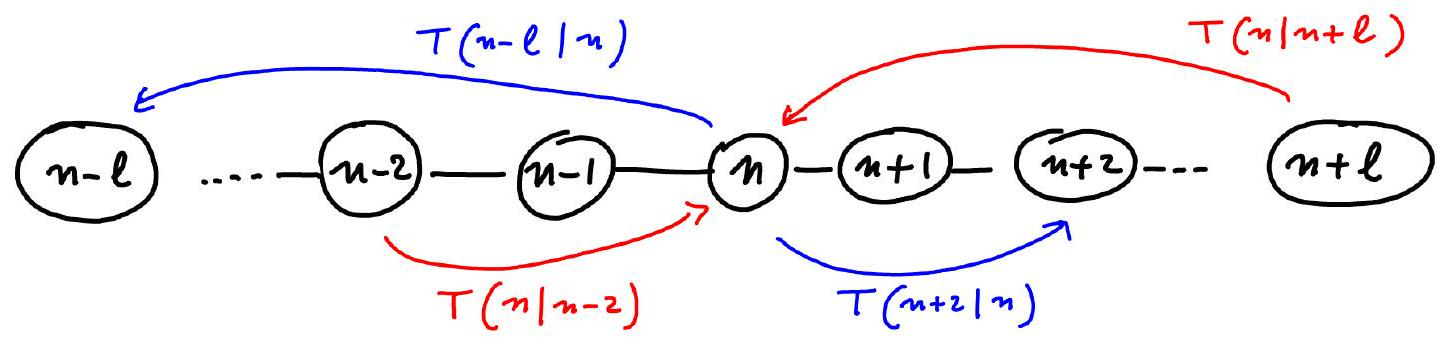
\includegraphics[width=0.5\textwidth]{2025_10_17_3daf2a002a8f5936c90eg-19}
\end{center}

The M.E. for the propogoton $p\left(n, t \mid n_{0}, t_{0}\right)$ is then
$P(n, t+\Delta t)=\underbrace{\sum_{m \neq n} T(n \mid m) \Delta t}_{\substack{\text { probability to } \\ \text { jump from any state } m \neq n \\ \text{ into the strete } n}} P(m, t)+\underbrace{\left(1-\sum_{m \neq n} T(m \mid n) \Delta t\right)}_{\substack{\text{probability to} \\ \text{zemain in the state } n}} P(n, t)$
Therefore as $\Delta t \rightarrow 0$ the Moster Equation becomes
(31) $\quad \frac{\partial}{\partial t} p(n, t)=\sum_{m}[T(n / m) p(m, t)-T(m / n) p(n, t)]$
notice that we have included the state $n$ in the sum (why?).

As usual e. (31) must be equipped with initial conditions $P\left(n, t_{0} \mid n_{0}, t_{0}\right)=\delta_{n, n 0}$ and, passibly, some boundory conditions.

Exercife: - Show that $\sum_{n} p(n, t)=1$.

\begin{itemize}
  \item Define the eth jump moment as
\end{itemize}

$$ \mu_{l}(n)=\sum_{m}(m-n)^{l} T(m / n) \quad l \geqslant 0 $$

Show then that

$$ \frac{d}{d t}\langle n\rangle=\left\langle\mu_{1}(n)\right\rangle \rightarrow \text { is this a closed ep. for }\langle n\rangle \text { ? } $$

$$ \frac{d}{d t}\left\langle n^{2}\right\rangle=\left\langle\mu_{2}(n)\right\rangle+2\left\langle n \mu_{1}(n)\right\rangle $$

where $\langle f(x)\rangle \equiv \sum_{x} f(x) p(x, t)$

As we have seen in ey. (40) and (46), we con define a matrix $\mathbb{W}$ whose entries are $(T(n \mid n)=0)$

$$ W_{n m}=T(n \mid m)-\sum_{l} T(l \mid n) \delta_{n, m} $$

which shows that $\mathbb{W}_{n m} \geq 0$ for $n \neq m$ and $\sum_{n} \mathbb{W}_{m m}=0$. The M.E. e. (31) then reads

$$ 
\begin{gathered}
\dot{\vec{p}}=W_{\vec{p}} \quad \text { or } \quad \dot{p}_{n}=\sum_{m} \mathbb{W}_{n m} p_{m} \\
\mathbb{W}=\left(\begin{array}{cccc}
 w_{11} & T(1 / 2) & T(1 / 3) & \ldots \\
 T(2 / 1) & w_{22} & T(2 / 3) & \ldots \\
 T(3 / 1) & T(3 / 2) & w_{33} & \\
 \vdots & \vdots & & \ddots
\end{array}\right) \leftarrow \text { jumps from } m=2,3 \ldots \text { to } 1 \\
 w_{ii} \equiv-\sum_{m} T(m \mid i) \\
 \substack{\text { jumps from } \\
 1 \text { to } m=2,3, \ldots}
\end{gathered}
$$ 

We con find the stationary state by setting $\dot{P}_{m}=0$ From ey. (31):
(32) $\quad \sum_{m}\left[T(n / m) p_{s t}(m, t)-T(m / n) p_{s t}(n, t)\right]=0$

This eg. is difficult to solve in general. However we con find the equilibrium salution if each and every term in the sum is zero (much stronger assumption). In this latter case we get

\section*{(33) $T(n \mid m) P_{\varphi}(m)=T(m \mid n) P_{\varphi}(n) \quad \text{DETAILED BALANCE}$}
This assumption means that every state $m$ is bolanced only by the state $n$, like in the birth
and death case, which in general is not true. All states are belonced in pairs. Of course, the detailed bolance condition satisfies ep. (32), but ep. (32) does not imply ey, (33). In general one cannot impose ep. (33).

We again con connect this to stat. Mech. If

$$ P_{\text {ep. }}(n)=\frac{1}{z} e^{-\beta E(n)}
$$ 
Where $E(n)$ is the energy of state $n$, then ep. (32) is satisfied if we choose $T(n \mid m)$ and $T(m \mid n)$ such that


\begin{equation*}
\frac{T(n \mid m)}{T(m \mid n)}=e^{-\beta(E(n)-E(m))} \tag{33}
\end{equation*}

Even though other choices are passible to satisfy detailed bolance, ep. (33) allows us to describe a physical system at equilibrium with a heat beth at temperature $\beta^{-1}$.
